\documentclass{ctexart}
\usepackage{tikz}
\usepackage{graphicx}
\usepackage[margin=2.5cm]{geometry}
\usetikzlibrary{patterns}

\begin{document}



\begin{figure}[htp]
    \centering
    \begin{tikzpicture}[>=latex]   
        \node (s1) at (0,0)[circle,draw=blue!50,fill=blue!20] {均方收敛};
        \node (s2) at (4,0)[rectangle,draw=blue!50,fill=blue!20] {已概率1收敛};
        \node (s3) at (2,-2)[rectangle,draw=blue!50,fill=blue!20] {低概率收敛};
        \node (s4) at (2,-4)[rectangle,draw=blue!50,fill=blue!20] {依分布收敛};
        \draw [->] (s1) -- (s3);
        \draw [->] (s2) -- (s3);
        \draw [->] (s3) -- (s4);
    \end{tikzpicture}
    \caption{框图}
\end{figure}

\begin{figure}[htp]
    \centering
    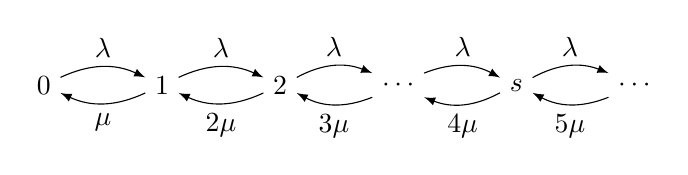
\begin{tikzpicture}[>=latex,scale=1.5]   
        \foreach \x/\xtext in {0/0,1/1,2/2,3/\cdots,4/s,5/\cdots}
        {
            \node (s\x) at (\x,0) {$\xtext$};
        }
        \draw[->](s0)to [bend left=25]node[above]{$\lambda$}(s1);
        \draw[->](s1)to [bend left=25]node[above]{$\lambda$}(s2);
        \draw[->](s2)to [bend left=25]node[above]{$\lambda$}(s3);
        \draw[->](s3)to [bend left=25]node[above]{$\lambda$}(s4);
        \draw[->](s4)to [bend left=25]node[above]{$\lambda$}(s5);

        \draw[<-](s0)to [bend right=25]node[below]{$\mu$}(s1);
        \draw[<-](s1)to [bend right=25]node[below]{$2\mu$}(s2);
        \draw[<-](s2)to [bend right=25]node[below]{$3\mu$}(s3);
        \draw[<-](s3)to [bend right=25]node[below]{$4\mu$}(s4);
        \draw[<-](s4)to [bend right=25]node[below]{$5\mu$}(s5);
    \end{tikzpicture}
    \caption{马尔可夫链}
\end{figure}

\begin{figure}[htp]
    \centering
    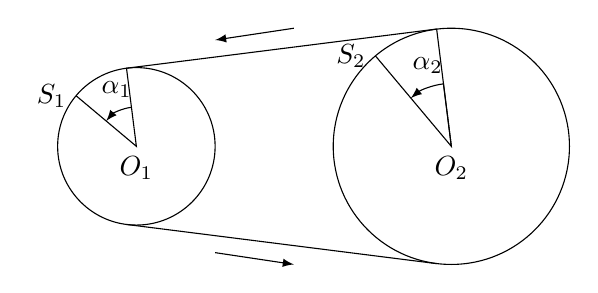
\begin{tikzpicture}[>=latex]   
        \draw (0,0)node[below]{$O_1$} circle(1);
        \draw (4,0)node[below]{$O_2$} circle(1.5);
        \draw (140:1)node[left]{$S_1$} -- (0,0) -- (97.2:1)--+(7.2:3.97)--(4,0)--+(130:1.5)node[left]{$S_2$};   % +坐标重置,以上个点为原点
        \draw (-97.2:1)--+(-7.2:3.97);  
        \draw[->] (97.2:.5) arc (97.2:140:0.5);
        \draw[->] (4,0)--+(97.2:0.8) arc (97.2:130:.8);

        \node at (-.25,.5)[above]{$\alpha_1$};
        \node at (4-.3,.8)[above]{$\alpha_2$};
        \draw[<-] (1,1.35)--(2,1.5);
        \draw[->] (1,-1.35)--(2,-1.5);
    \end{tikzpicture}
    \caption{坐标重置}
\end{figure}

\begin{figure}[htp]
    \centering
    \begin{tikzpicture}[>=latex]   
        \begin{scope}
            \draw[->] (-1.5,0)--(1.5,0)node[right]{$x$};
            \draw[->] (0,-1.5)--(0,1.5)node[right]{$y$};
            \draw (0,0) circle(1);
            \node at (.25,.25){$O$};
            \foreach \x/\xcorr in {+/{.5,.5},-/{-.5,.5},-/{-.5,-.5},+/{.5,-.5}}
            {
                \node at (\xcorr) {$\x$};
            }
            \node at (0,-2) {$\cos\alpha$和$\sec\alpha$};
        \end{scope}
        \begin{scope}[xshift=4cm]
            \draw[->] (-1.5,0)--(1.5,0)node[right]{$x$};
            \draw[->] (0,-1.5)--(0,1.5)node[right]{$y$};
            \draw (0,0) circle(1);
            \node at (.25,.25){$O$};
            \foreach \x/\xcorr in {+/{.5,.5},+/{-.5,.5},-/{-.5,-.5},-/{.5,-.5}}
            {
                \node at (\xcorr) {$\x$};
            }
            \node at (0,-2) {$\sin\alpha$和$\csc\alpha$};
        \end{scope}
        \begin{scope}[xshift=8cm]
            \draw[->] (-1.5,0)--(1.5,0)node[right]{$x$};
            \draw[->] (0,-1.5)--(0,1.5)node[right]{$y$};
            \draw (0,0) circle(1);
            \node at (.25,.25){$O$};
            \foreach \x/\xcorr in {+/{.5,.5},-/{-.5,.5},+/{-.5,-.5},-/{.5,-.5}}
            {
                \node at (\xcorr) {$\x$};
            }
            \node at (0,-2) {$\tan\alpha$和$\cot\alpha$};
        \end{scope}
    \end{tikzpicture}
    \caption{多张图片的布局}
\end{figure}

\begin{figure}[htp]
    \centering
    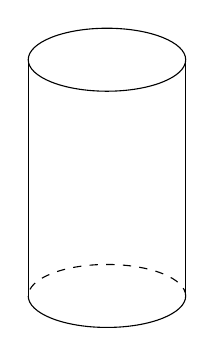
\begin{tikzpicture}[>=latex]   
        \draw (-1,0) -- (-1,3);
        \draw (1,0) -- (1,3);
        \draw (0,3) ellipse [x radius=1,y radius=.4];
        \draw[dashed] (1,0) arc [start angle =0,end angle = 180, x radius=1,y radius=.4] ;
        \draw (1,0) arc [start angle =0,end angle = -180, x radius=1,y radius=.4] ;
    \end{tikzpicture}
    \caption{绘制圆柱体}
\end{figure}

\end{document}